\documentclass{article}
\usepackage{amsmath, amssymb, cite, algorithmic, url, braket}
\usepackage{graphicx}
\usepackage{pythonhighlight}
\usepackage[margin=1.5cm]{geometry}
\usepackage[title]{appendix}
\usepackage{subfigure}
\usepackage{listings}
\usepackage{booktabs}

\graphicspath{{../pic/}}
\lstset{
language=[ANSI]{C},
showtabs=true,
tab=,
tabsize=2,
basicstyle=\ttfamily\footnotesize,%\setstretch{.5},
stringstyle=\color{stringcolour},
showstringspaces=false,
alsoletter={1234567890},
otherkeywords={\%, \}, \{, \&, \|},
keywordstyle=\color{keywordcolour}\bfseries,
upquote=true,
morecomment=[s]{/*}{*/},
commentstyle=\color{commentcolour}\slshape,
literate=*%
{=}{{\literatecolour=}}{1}%
{-}{{\literatecolour-}}{1}%
{+}{{\literatecolour+}}{1}%
{*}{{\literatecolour*}}{1}%
{!}{{\literatecolour!}}{1}%
{[}{{\literatecolour[}}{1}%
{]}{{\literatecolour]}}{1}%
{<}{{\literatecolour<}}{1}%
{>}{{\literatecolour>}}{1}%
% {>>>}{\pythonprompt}{3}%
,%
frame=trbl,
rulecolor=\color{black!40},
backgroundcolor=\color{white},
breakindent=.5\textwidth,frame=single,breaklines=true
}

\begin{document}
\title{DSP Homework 12}
\author{Xu, Minhuan}
\maketitle
\tableofcontents
\begin{abstract}
In the first section, I summarized the videos we watched in class this week. There are two topics, IPv6 and SDR. I put forward my own ideas on these two topics. In the second section, I measured the highest frequency and lowest frequency of my voice by using the filter to continuously test. In the third section, I try to use the knowledge of information theory to explain why the phase spectrum of an image contains more information.
\end{abstract}



\section{Videos}
\subsection{SDR}
This video introduced three parts of the SDR (Software-defined Radio), which is SDR receiver, antenna and computer software. Interesting one of the three is the RTL receiver which is a RTL-level circuit which make the EM wave it received into digital signals. 

As an introduction video, this video teach us how to judge the 3 parts' performance. First, the noise, this is common. Second, TCXO, representing the shift when the temperature changes, usually, the smaller, the better. Third, bandwidth, it is important if we want to listen to more channels.

For antennas, there are discore antenna, vertical antenna, magmount car antenna and DIY antenna. First two antennas are not suitable for beginners, because the former is not specially tuned, and the latter should be set up outside. If we students want to receive the radio using antenna, the magmount car antennas or DIY antenna are good for beginners.

\subsection{IPv6}
We are stepping into the era of IPv6. IPv4 has $2^32$ addresses, but this is not enough for today's devices, so there's IPv6. IPv6 uses $128 ~$ bits to represent an address, so there are much more addresses to meet the increasing requirement.

The IPv6 addresses are too long so that we need use some trick to shorten them. We can use "::" to represent several "0000", and we can ignore '0's if it don't influence the value, which means highest '0's.

The subnet mask in IPv4 is used to specify the subnet, but in IPv6, there's no subnet mask, but use the forward slash to represent the same meaning. For example, $/4$ represent the first $4$ bits in the address. Moreover, the IPv6 addresses are also classified into several groups, such as, 2000::/3 represent the highest 3 bits of 2000, and this prefix means global unicast, like the public IP in IPv4.

\subsection{My Thoughts}
\subsubsection*{SDR}
Actually, we made a box antenna in last summer holiday lessons, that is interesting to make an antenna and test it using the equipment. I have thought about using that DIY antenna to send something, and I have known a little about the SDR before. I want to try to explore how the SDR if I have the chance.
\subsubsection*{IPv6}
I am very glad to see the IPv6 is developing.If every device can have its own address, it will be much convenient to play video games together or host a server of, perhaps, Minecraft, which is a customizable java game. Moreover, the smart devices around us can 'talk' with each other, so that they can work better.

\section{Frequency Range of Voice}
To find the range of my voice frequency, I want to record my voice and do FFT to it. Then, I filter some frequencies under or beyond a certain value, if I can hear my voice, I filter more frequencies out until I cannot hear my voice. See Fig.~\ref{fig:voiceSpectrum}, there are the original wave, wave through a high-pass filter and spectrum of the 2nd wave.

\begin{figure}[!h]
	\centering
	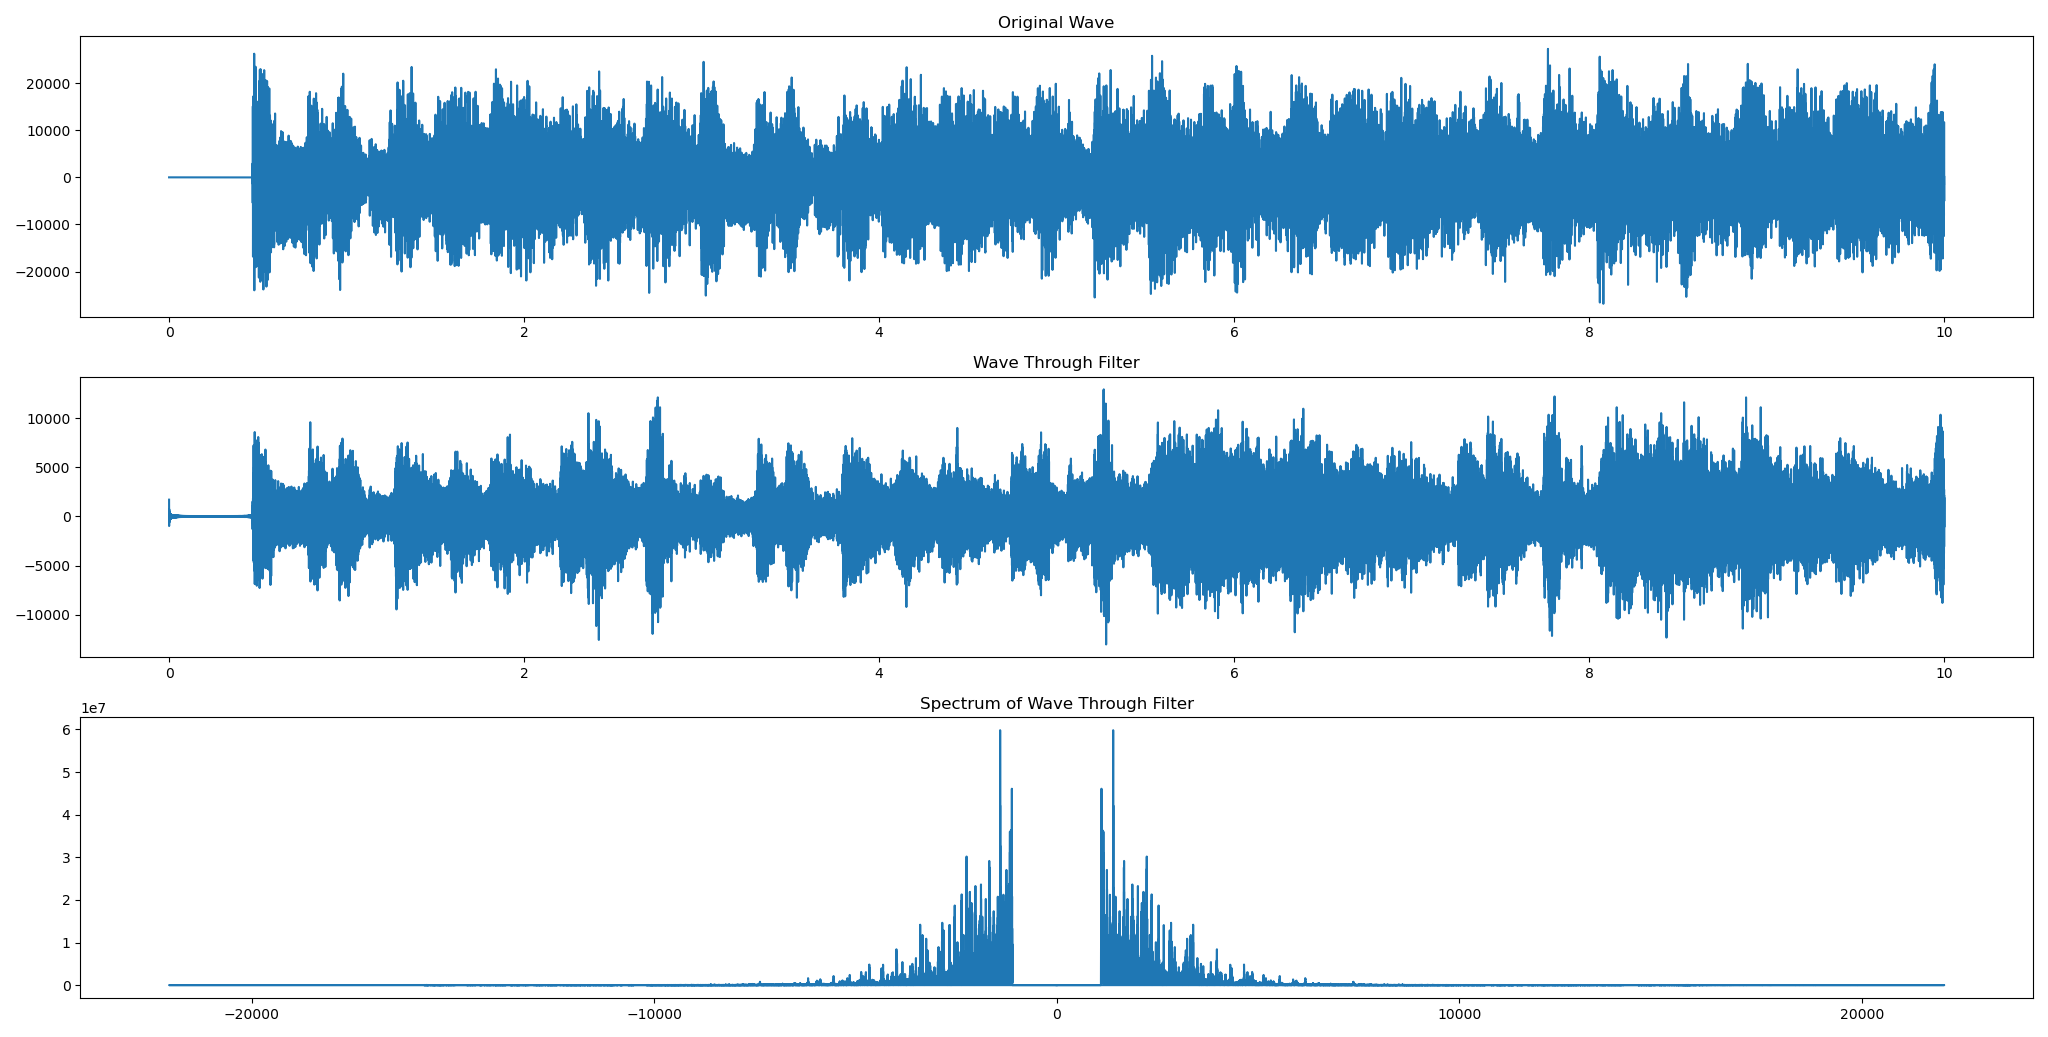
\includegraphics[width=6 in]{../pic/voiceSpectrum.png}
	\caption{Spectrum of My Voice}
	\label{fig:voiceSpectrum}
\end{figure}

\section{Which Contains More Image Information, Amplitude or Phase?}
\subsection{Explanation}
It is the phase which contains more information. We can see from the FFT spectrum that the amplitude is more in order, and the phase is more in disorder. Because of the definition of the information entropy, the more \emph{chaotic} the signal, the \emph{more information} it contains. And the specific phenomenon is that there will be greater difference between signals containing more information.



To prove my idea, I found 2 pictures to have an experiment. I calculate the amplitude and the phase of the 2 pictures and calculate the correlation coefficients. I draw those pictures as below, see Fig.~\ref{fig:imgSpec}. It is easy to find that the correlation coefficient of phase is much smaller than that of amplitude. And I calculate the summations of the correlation coefficients of amplitude and phase, they are respectively about 1.8 million and about 5.6 thousand, see Fig.~\ref{fig:corrcoef}. They are not on the same order of magnitude.

\begin{figure}[!h]
	\centering
	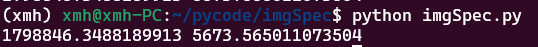
\includegraphics[width=3 in]{../pic/corrcoef.png}
	\caption{Comparison of Correlation Coefficients}
	\label{fig:corrcoef}
\end{figure}

I guess the reason why the amplitude contains less information is amplitude spectrum only contains how fast the pixels are changing compared with the pixels around them, because pictures composed of pixels must be readable, pixels won't change too fast and the frequency are almost the same between readable pictures. But the phase contains how the pixels change compared with pixels around, so it can contain more visible information compared to the amplitude.

\begin{figure}[!h]
	\centering
	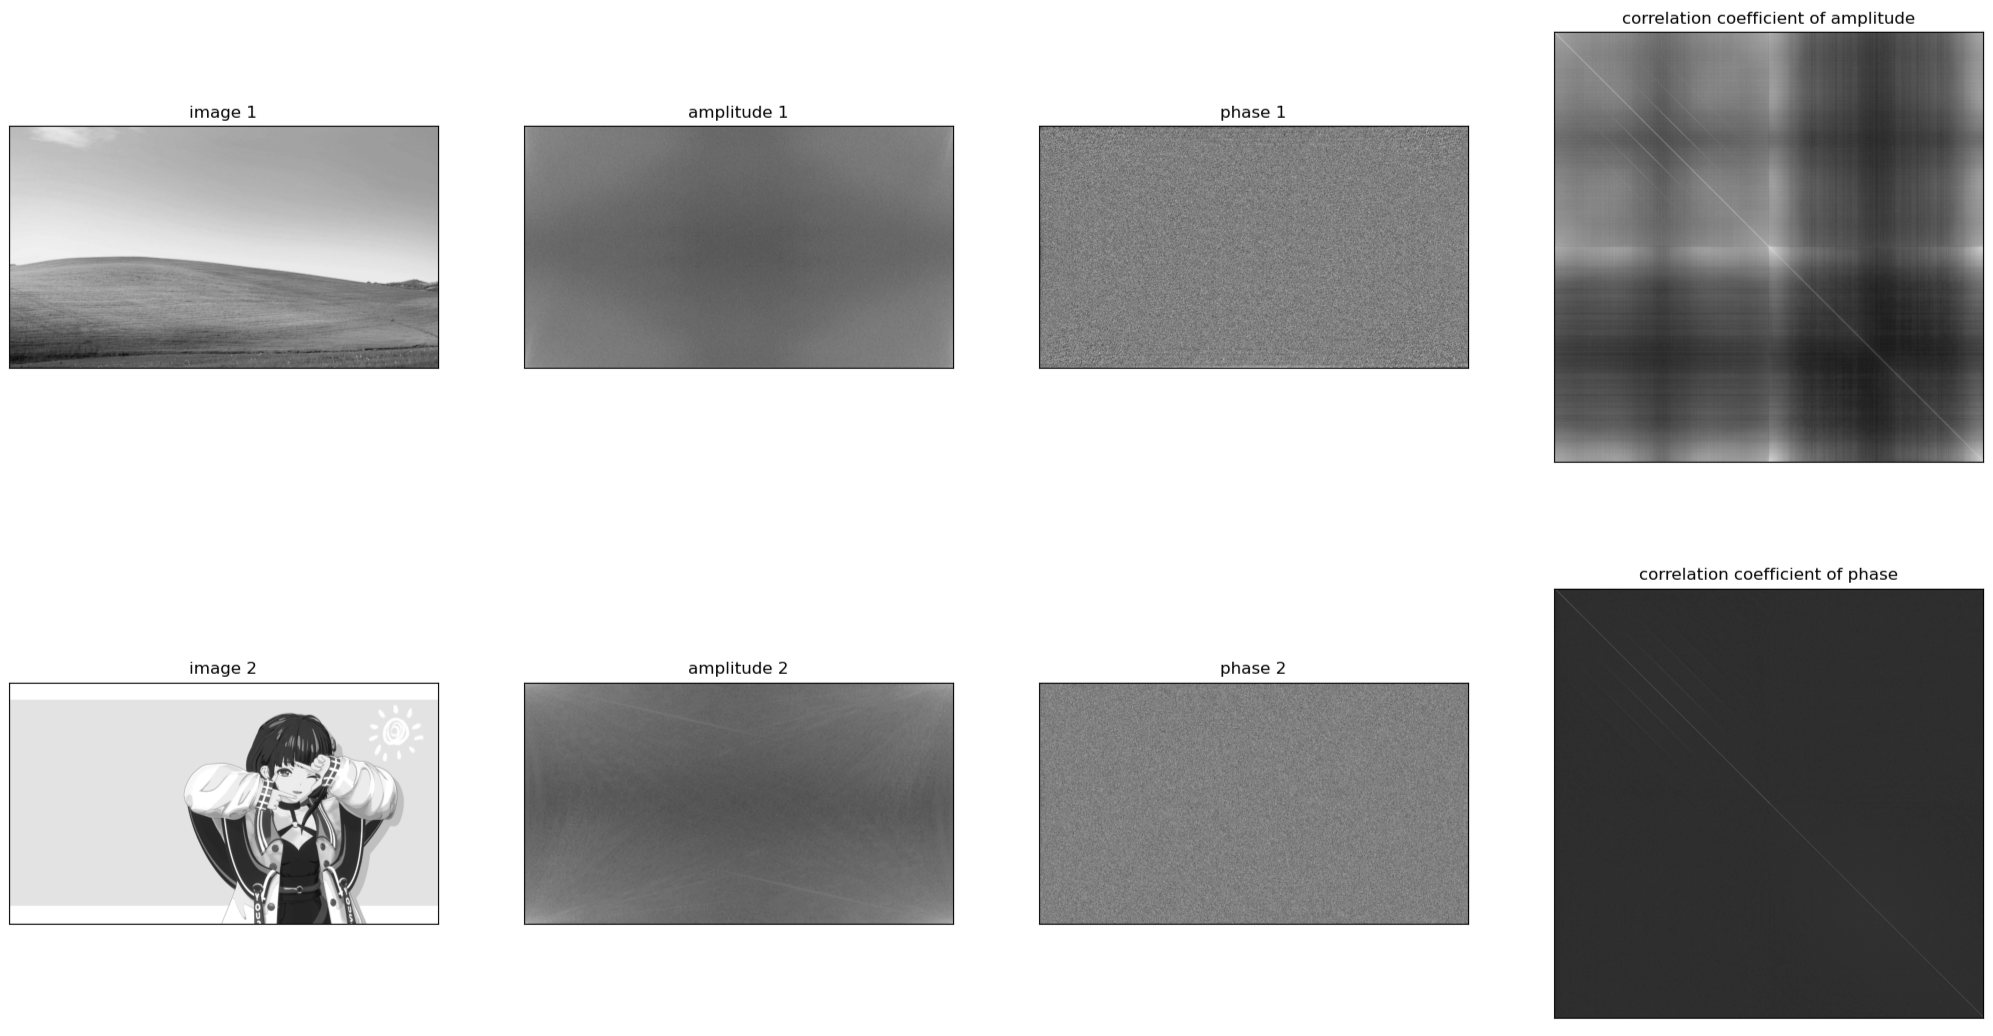
\includegraphics[width=6 in]{../pic/imgSpec.png}
	\caption{Spectrum and Correlation Coefficients of Two Pictures}
	\label{fig:imgSpec}
\end{figure}


\bibliographystyle{ieeetr}
\bibliography{../bib/database}

\begin{appendices}
\section{Code Listing}
\begin{python}
# voice.py
import numpy as np
from numpy.fft import fft, fftfreq, ifft
from matplotlib import pyplot as plt
from scipy.io.wavfile import write, read

"""Read Record File"""
fs, x = read('song.wav')
x = x[:, 0]
sec = x.size/fs
t = np.arange(0, sec, 1/fs)

"""Do FFT"""
xt = fft(x)
ap = np.abs(xt)
phase = np.angle(xt)
freq = fftfreq(x.size, d=(1/fs))

"""Simple High-Pass Filter"""
fc = 1100
ap[int(-fc * sec):] = 0
ap[:int(fc * sec)] = 0
"""Simple Low-Pass Filter"""
# cfq = xt.size/2
# ap[int(cfq - (fs/2 - 2000) * seconds):int(cfq + (fs/2 - 2000) * seconds)] = 0

"""Do IFFT And Output"""
xt_f = ap * np.exp(1j * phase)
ix = np.real(ifft(xt_f))
write('out.wav', fs, ix)

"""Draw Wave and Spectrum"""
ax0 = plt.subplot(311)
ax0.set_title("Original Wave")
ax0.plot(t, x)

ax1 = plt.subplot(312) 
ax1.set_title("Wave Through Filter")
ax1.plot(t, ix)

ax2 = plt.subplot(313)
ax2.set_title("Spectrum of Wave Through Filter")
ax2.plot(freq, ap)

plt.show()

\end{python}

\begin{python}
# imgSpec.py
import cv2
import numpy as np 
from matplotlib import pyplot as plt

img1 = cv2.imread("bliss.jpeg", cv2.IMREAD_GRAYSCALE)
imgt1 = np.fft.fft2(img1)
img2 = cv2.imread("yousa.jpg", cv2.IMREAD_GRAYSCALE)
imgt2 = np.fft.fft2(img2)

amp1 = np.log(abs(imgt1))
pha1 = np.angle(imgt1)
amp2 = np.log(abs(imgt2))
pha2 = np.angle(imgt2)

corr_amp = np.corrcoef(amp1, amp2)
corr_pha = np.corrcoef(pha1, pha2)
print(np.sum(corr_amp), np.sum(corr_pha))

imgs = ['img1', 'amp1', 'pha1', 'corr_amp', 'img2', 'amp2', 'pha2', 'corr_pha']
names = ['image 1', 'amplitude 1', 'phase 1', 'correlation coefficient of amplitude', 'image 2', 'amplitude 2', 'phase 2', 'correlation coefficient of phase']

plt.figure()
for i in range(len(imgs)):
    ax=plt.subplot(2, 4, i + 1, xticks=[], yticks=[])
    ax.set_title(names[i])
    ax.imshow(eval(imgs[i]), cmap='gray')
plt.show()
\end{python}
\end{appendices}

\end{document}